\subsubsection{Frustration} \label{frust-4}


Wie bereits in Abschnitt 7.3.3 dargeboten, stellt die Frustration einen negativen Zustand des Menschen dar, welcher durch Misserfolgserlebnissesowie durch Versagungs- und Entt{\"a}uschungserlebnisse einhergehen kann. Die Frustration stellt einen negativen Zustand des Menschen dar, welcher mehrere Indikatoren haben kann. Dieser Zustand kann sowohl eine Gef{\"u}hlslage als auch eine Folge vorhergehender Emotionen sein. \\

F{\"u}r das Frustrationsexpermiment der Studie soll erneut auf das Ausl{\"o}sen der Misserfolgserlebnisse sowie eine empfundene Ungerechtigkeit zur{\"u}ckgegriffen werden. \\



\begin{figure}[H] \centering
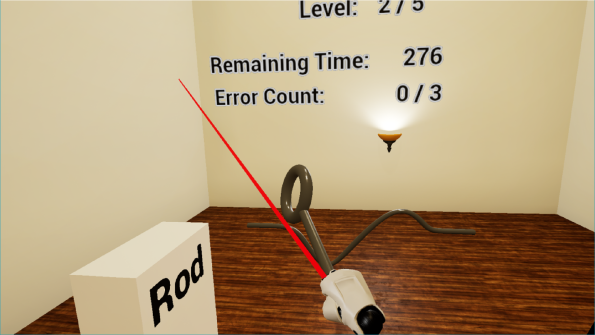
\includegraphics[width=\textwidth]{Images/frust4.png} 
\caption{ Bild des Frustrations-Szenarios in VR. }
\label{fig:frust4} 
\end{figure}




Dem Probanden wird die Aufgabe gestellt, in eine VR-Umgebung das Spiel ``hei{\ss}er Draht'' zu spielen. In diesem Spiel besteht die Aufgabe darin, den Ring, welcher sich in der Hand des Spieler befindet, von dem Startpunkt zum Endpunkt eines Drahts zu bef{\"o}rdern. Der Ring darf w{\"a}hrenddessen den Draht nicht ber{\"u}hren.Dieses Spiel ist durch die geschwungene Form des Drahts schwierig und fordert daher viel Ruhe und Geschick. Dem Probanden wird eine Zeit vorgegeben, in welcher dieser von dem Startpunkt zum Endpunkt gelangen muss. Der Faktor des Zeitdrucks kann eine Stressreaktion ausl{\"o}sen. Da das Spiel jedoch den Ehrgeiz erwecken kann, kann es dazu f{\"u}hren, dass es nicht zu der erhofften Frustration kommt. Um diese Emotion trotzdem einleiten zu k{\"o}nnen, wird das Spiel an einigen Stellen so prepariert, dass der Proband durch Spielfehler den Draht ber{\"u}hrt und erneut von dem Startpunkt aus starten muss. Die empfundene Ungerechtigkeit und Ohnm{\"a}chtigkeit des Probanden soll als Indikator der Frustration dienen.
